\subsection{question 3: Find leading indicators and predict swings}

\subsubsection{Measure Swing}
As stated in the problem, what needs to be predicted is the swings of the match. So we came up with a way to quantify the swings. 
\begin{figure}[bt!]
    \centering
    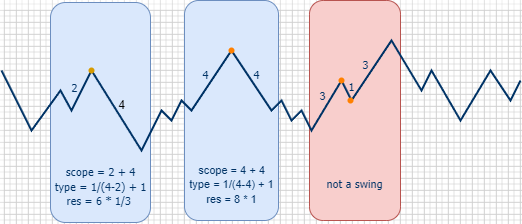
\includegraphics[width=0.75\linewidth]{figure/convert.drawio.png}
    \caption{\centering Swing Measurement}
    \label{fig:swingM}
\end{figure}
As shown in figure \ref{fig:swingM}, we use folded lines to demonstrate the game's flow. The impact of swing is divided into 2 parts:
\begin{itemize}
    \item \textbf{Scope: }Sum the lengths of the folded lines, then Find the kth power(k is used to measure the influence of the scope factor)
    \item \textbf{Type: }In figure \ref{fig:swingM}, (a) only scored 2 points in a row before experiencing a 4-game losing streak, whereas (b) was on a winning streak before the losing streak, suggests that the turning point in (b)'s situation had a greater impact. The difference in the lengths of the 2 folds should be inversely correlated with the measure, so we use the inverse proportion function.
\end{itemize}

Combining the 2 factors, the final equation is equation (\ref{equ:convert}). 
\begin{equation}
    impact = (l+r)^k \cdot \frac{1}{|l-r|+1}
    \label{equ:convert}
\end{equation}

\subsubsection{Decision Tree}
To determine the critical game indicators, we utilize the decision tree to capture various data throughout the game. \par

Decision Tree (DT) is non-parametric supervised learning that can summarize the decision rules from a series of featured and labeled data to solve classification or regression problems. \par
Meng and Huang \cite{ref1} used a decision tree model in the quantitative analysis of players' winning factors and concluded that the most important winning factor in women's tennis is the serving situation as well and the reduction of forced errors is the main way to improve the winning rate of the game. 
We took inspiration from this and used a decision tree model to predict turning points in the game while deriving the feature importance of each indicator. \par
Details about the model: 
\begin{itemize}
    \item \textbf{Gini Coefficient: }
    Using the decision tree model based on the CART algorithm for prediction, due to the use of the information entropy and the Gini coefficient of the effect is basically the same, but the calculation of the information entropy is more complex than the Gini coefficient, in addition to high-dimensional data or more noisy data, the information entropy is very easy to overfitting\cite{ref2}. Therefore, we use the Gini coefficient (gini) as a criterion parameter, the Gini coefficient (gini) index to measure the degree of stochasticity, it is defined in equation \ref{equ:dt1}
    \begin{equation}
        Gini(t) = 1- \sum_{i=0}^{c-1}{p(i|t)^2}
        \label{equ:dt1}
    \end{equation}
    \item Increase tree depth, decrease leaf nodes due to small sample size and large number of features. Higher accuracy was achieved with a maximum tree depth of 15 and 30 maximum leaf nodes.
    \item \textbf{Feature Importance: }Use Gini coefficient to determine indicator importance for the decision tree. The equation is \ref{equ:dt2}

    \begin{equation}
        I(feature)=\sum^n_{i-1}{\frac{filtered\_samples}{total\_samples}gini\_gain(decision\_node)}
        \label{equ:dt2}
    \end{equation}
    
\end{itemize}

The calculated data are normalized to obtain the characteristic importance of each indicator, which is partially plotted in figure \ref{fig:dt1}. Based on the figure, the most essential features are server, score, and point victor. These indicators have a significant impact on the game's volatility.\par


\begin{figure}[bt!]
    \centering
    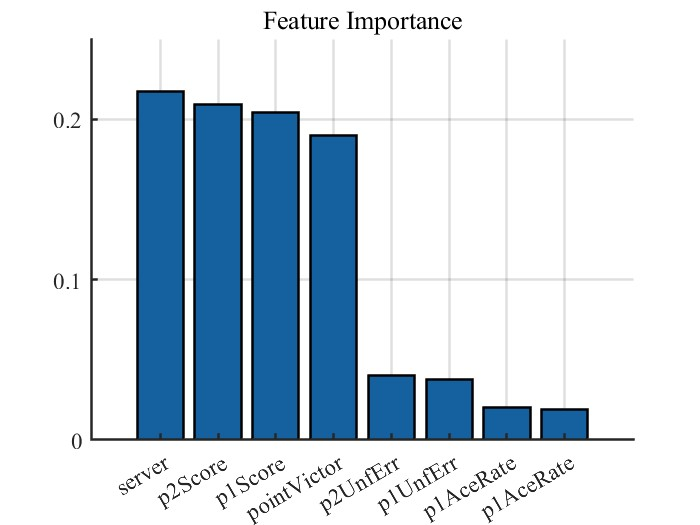
\includegraphics[width=0.6\linewidth]{figure/dt1.jpg}
    \caption{\centering Decision Tree Main Indicators}
    \label{fig:dt1}
\end{figure}

\subsubsection{Decision Tree Experiment}
\begin{table}[b!]                    % [] control the position of table
\caption{\centering Decision Tree Evaluation}
    \centering
    % \renewcommand{\arraystretch}{1.5}
    \begin{tabular}{c c c c c }            % main part of table: {} control alignment(c c c c c )
        \toprule 
        
          & \multicolumn{1}{l}{Accuracy} & \multicolumn{1}{l}{recall} & \multicolumn{1}{l}{Precision} & \multicolumn{1}{l}{F1} \\
        \midrule
    Train   & 0.77 & 0.77 & 0.75 & 0.754 \\
    Test   & 0.75 & 0.75 & 0.725 & 0.73 \\

        \bottomrule
    \end{tabular}
    \vspace{10pt}
    \vspace{-5pt}
    \label{tab:dt1}
\end{table}

\subsubsection{LSTM Specific to The Problem}
After obtaining the primary INDICATORS using the decision tree, we replace the model inputs in LSTM with the simple processed data corresponding to those INDICATORS. Upon completion of the training, we achieved an accuracy of 0.7, which is a remarkable outcome and in accordance with our initial expectations. This result verifies that we have identified the correct and efficient indicators. However, we would like to point out that Question 3 does not require us to predict the outcome of the game but rather the swing of the game.\par
After analyzing the problem, the swing was first quantified (), followed by some adjustments to the LSTM model based on the characteristics of the problem: \par 
\begin{figure}[bt!]
    \centering
    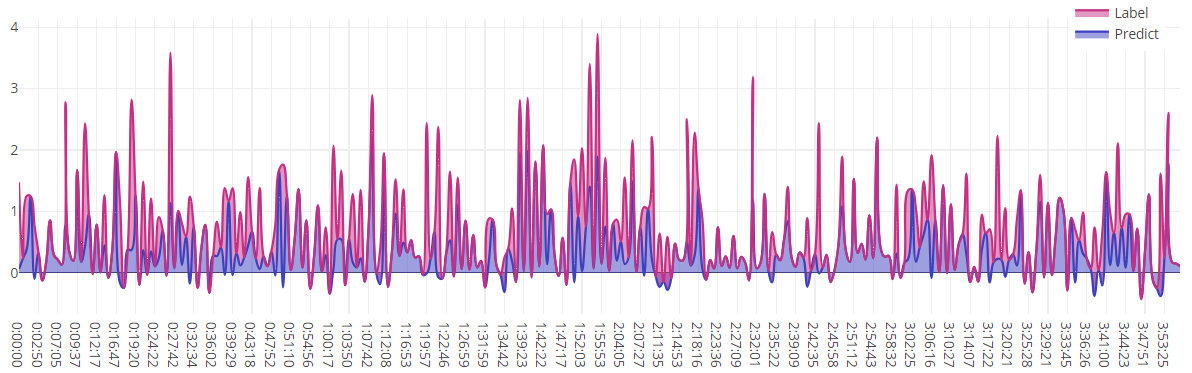
\includegraphics[width=1\linewidth]{figure/lstm2.png}
    \caption{\centering LSTM Prediction}
    \label{fig:lstm2}
\end{figure}
\begin{itemize}
    \item \textbf{Regression Model: }
    In the initial model, the problem is treated as a regression problem to predict values close to our quantized swing values. The predictions obtained by the trained model are illustrated in Figure \ref{fig:lstm2}.
    \item \textbf{Transforms Into a Categorization Problem at Output:}
    \begin{itemize}
        \item \textbf{Why?}
        We believe that for this problem, the regression problem is clearly more difficult compared to the classification problem.
        The regression model uses Mean Squared Error (MSE) as the loss function. To evaluate the effectiveness of the MSELoss, we must consider the data range. And MSELoss is less intuitive than accuracy.
        \item \textbf{How?}
        During training, we still train the model as a regression model to take advantage of the benefits offered by quantized turning points but transform the model output into a classification. Details: Set the value that is not a turning point to 0 and make the turning point value converge to 1 using the equation (\ref{equ:lstm2}). In the output, we transform the model prediction into 0/1. If it is a test, you need to do the label accordingly.
        \begin{equation}
            swing\_label =\begin{cases} sigmoid(swing)\quad ,swing>0 \\0\quad,swing=0 \end{cases}  
            \label{equ:lstm2}
        \end{equation}
    \end{itemize}
    
\end{itemize}
\begin{figure}[bt!]
    \centering
    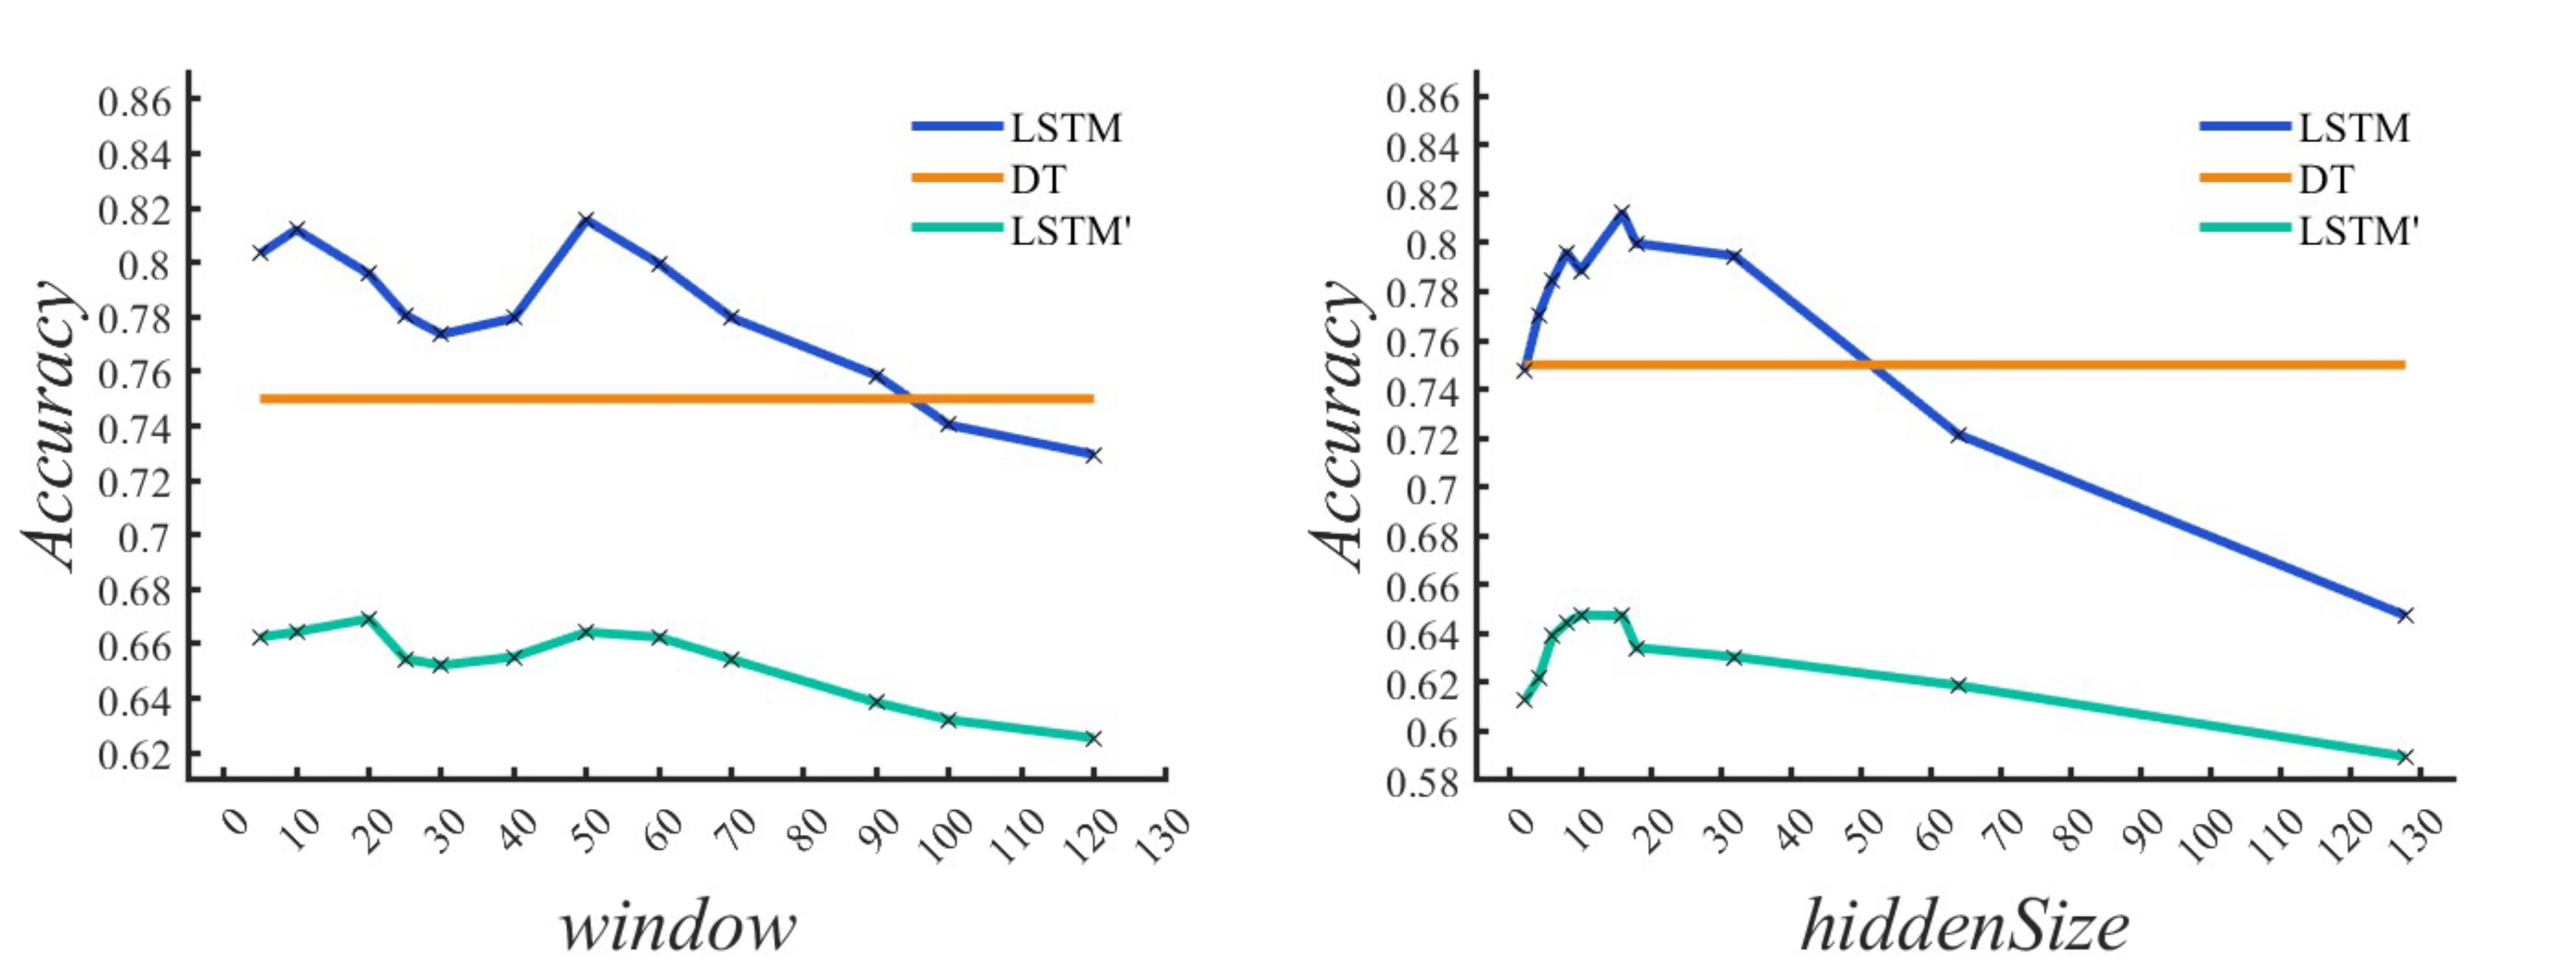
\includegraphics[width=1\linewidth]{figure/lstm3.png}
    \caption{\centering Adjusted LSTM Experiment\\
    \vspace{2pt}
    (LSTM: use main indicators as input, LSTM': remove main indicators)}
    \label{fig:lstm3}
\end{figure}
The results of some of our experiments are shown in Figure \ref{fig:lstm3}, where the best model achieves an accuracy of \textbf{0.81} and the model without using main indicators as input perform poorly. This indicates that we chose the right indicators in the decision tree part and the success of the adjustment we've made to the lstm model as described above.

\subsubsection{Discussion}
\textbf{Window Size: }
    We further discussed the window size discussed in question 2. In the model built in question 3, window size has an impact on model performance, which indicates that the model built in question 3 makes better use of the LSTM's advantage, which is utilizing long and short-term memory. It also suggested that for the LSTM model, the raw data should not be processed too much, which is more favorable for the model to obtain information.

\subsubsection{Suggestions}
Based on the statistics we've got, Athletes need to focus on the influences of the serve, the game situation, the winner of the previous game, etc., during the match. We also experimented with the influence of different situations through the Decision Tree. For example, we tested whether a score of 40 plays a more important role than a score of 30. The results show that there is very little difference in their impact and it depends on the players' own characteristics. Different players react differently to the same situation. \par

We recommend focusing on these main factors and designing tactics with his characteristics. Maximize the duration of his side's advantage and minimize fluctuations in the game that are not in his favor. \par

